\documentclass[a4paper,12pt]{article}

\usepackage{graphicx}
\usepackage{amsmath}
\usepackage{hyperref}
\usepackage{caption}
\usepackage{subcaption}
\usepackage{circuitikz}

\title{\textbf{Lab Report: Experiment 2}}
\author{EE24BTECH11003 : Akshara Sarma Chennubhatla\\EE24BTECH11005 : Arjun Pavanje}

\begin{document}
\maketitle
\begin{center}
	\textbf{Experiment:}\\Studying the transient\\and steady state response\\of an RC Circuit\\with Square Wave Input
\end{center}
\vspace{30pt}
\begin{figure}[h!]
	\centering
	
\includegraphics[width = 100pt]{.logo/logo.png}\\
\end{figure}
\begin{center}
	Bachelor of Technology\\
	\vspace{10pt}
	Department of Electrical Engineering\\
\end{center}
\newpage
\section*{Objective}

To analyze the transient and steady-state responses of an RC circuit to a square wave input $(0-5V)$ in three cases: \newline
\begin{enumerate}
	\item $RC << T$\\
	\item $RC = T$\\
	\item $RC >> T$
\end{enumerate}
where $T$ is the time period of the input square wave.


\section*{Equipment Used}
\begin{itemize}
	\item Function generator
	\item Resistor $R$
	\item Capacitor $C$
	\item Oscilloscope
	\item Wires
	\item Breadboard
\end{itemize}

\section*{Theory}
\pagebreak
\begin{figure}[h!]
    \centering
    \begin{circuitikz}
        \draw
        (0,0) node[ground] {}
        to[vsourcesquare, l=\( 5V\)] (0,3) -- (1,3)
        to[R, l=\(R\)] (3,3)
        to[short] (3,2)
        to[C, l=\(C\)] (3,0) -- (0,0);
    \end{circuitikz}
    \caption{RC Circuit}
    \label{fig:circuit}
\end{figure}
Governing equation of the above RC circuit is,
\begin{align}
  iR + V_c = V(t)\\
  C\frac{dV_c}{dt}R + V_c = V(t)\\
  \frac{dV_c}{dt} = \frac{1}{RC}(V(t) - V_c)  
\end{align}
Now we can apply any of the known methods for numerically solving differential equations (such as Euler's Method, Backward Euler's Method, Runge-Kutta Method, Trapezoidal Rule). Here, we have chosen to use Trapezoidal rule. 
\begin{align}
	\int_{x_n}^{x_{n+1}}dV_c &= \frac{1}{RC} (\int_{x_n}^{x_{n+1}}V(t)dt - \int_{x_n}^{x_{n+1}}V_c dt)\\
  V_c(t_{n+1}) - V_c(t_n) &= \frac{1}{RC}\left(\frac{h}{2}(V(t_{n+1} + V(t_n))) + \frac{h}{2}(V_c(t_{n+1}) + V_c(t_n))    \right)
\end{align}
This simplifies to be,
\begin{align}
  V_c(t_{n+1}) = V_c(t_n)\left(\frac{2RC-h}{2RC+h}\right) + \frac{h}{2RC+h}(V(t_{n+1}) +V(t_n))
\end{align}

\section*{Procedure}

\subsection*{Connecting Circuit}
\pagebreak
\begin{figure}[h!]
	\centering
	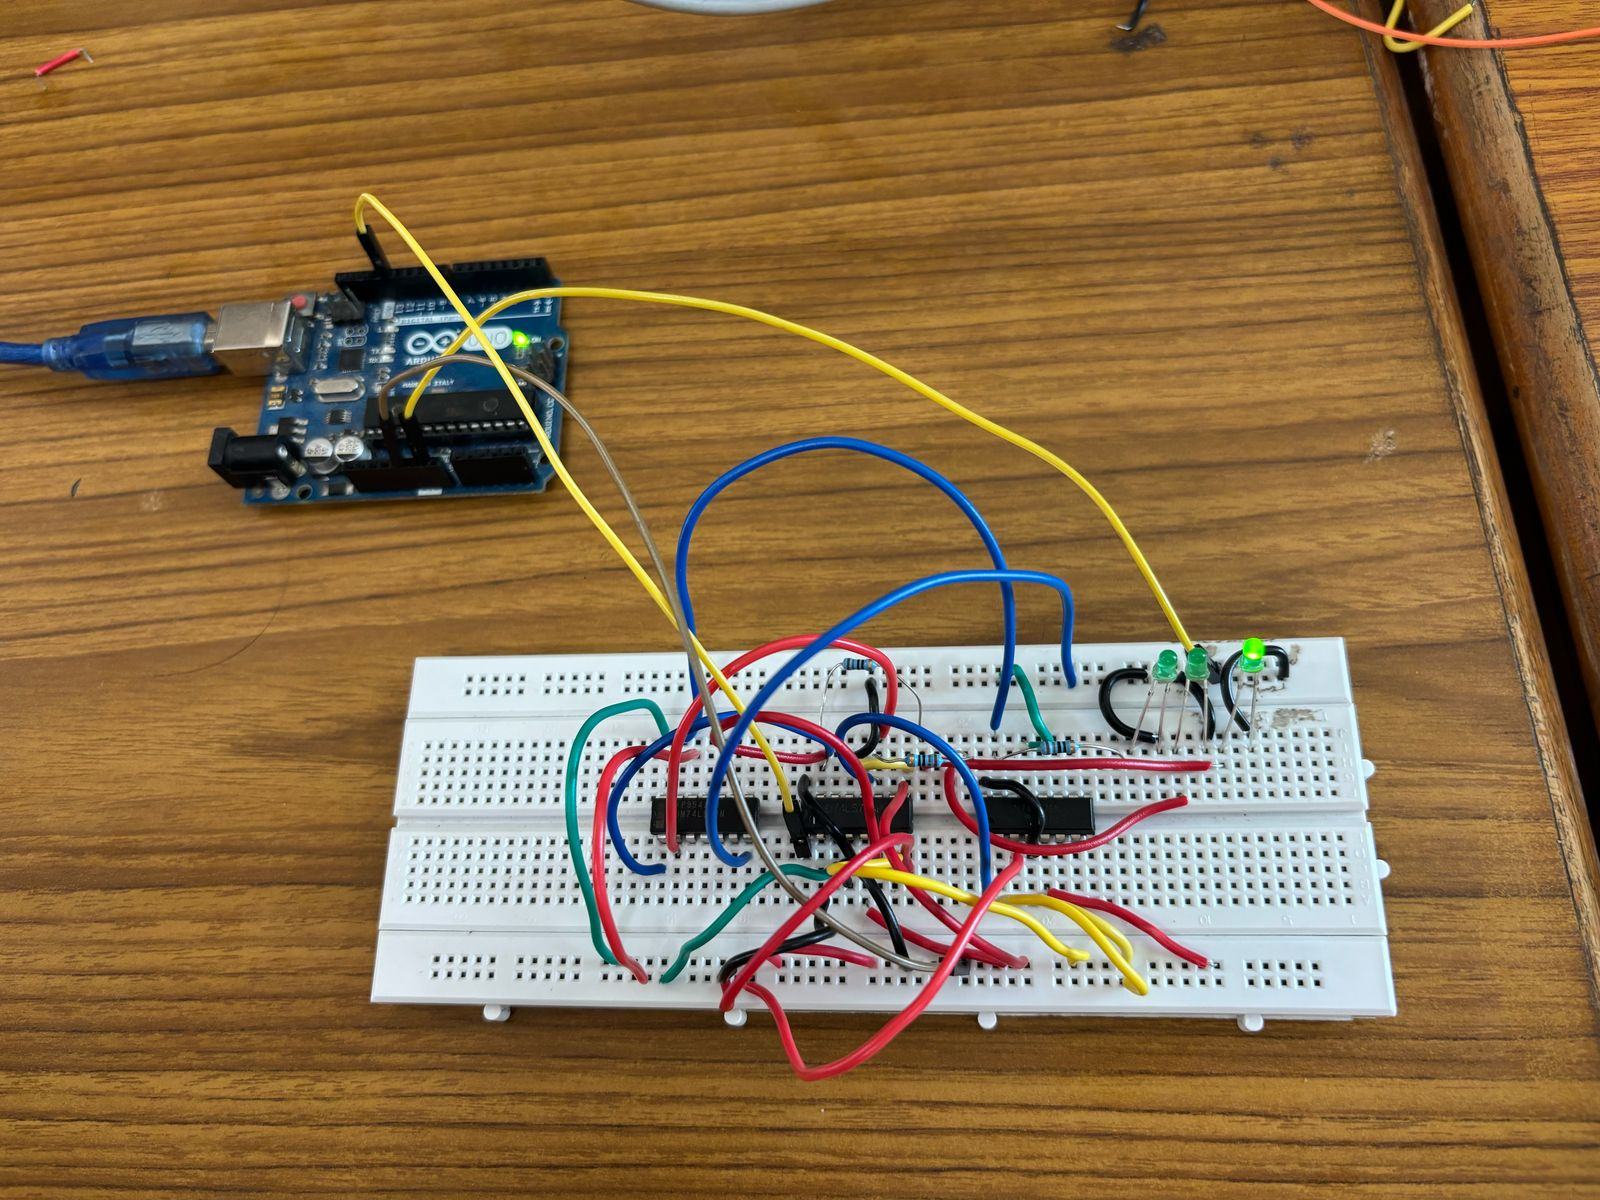
\includegraphics[width = 300pt]{figs/circuit.jpg}
\end{figure}

\begin{enumerate}
	\item Construct the circuit as shown in the above figure.
		\begin{enumerate}
			\item Connect the positive end of the function generator in series with a resistor
		\end{enumerate}
	\item Set the function generator to output a square wave with $5V$ amplitude (Peak Voltage $5V$, Minimum Voltage $0V$) and a time-period $T$.
		Select the type of cycle as \textit{N-CYCLES}.
	\item Connect the second channel of the function generator to the second channel of the oscilloscope. Set the waveform for this as a square wave with the same conditions as in the first channel. This will allow us to compare output voltage across capacitor with input square wave.
	\item This configuration enables the generation of a square wave with a predefined number of cycles when the trigger button is pressed on the function generator.
		On the oscilloscope, press the \textit{SINGLE} button. This ensures that the next event captured by the oscilloscope is displayed and then the display pauses automatically.
	\item Trigger the burst mode manually on the function generator to generate the single pulse or event.
	\item Observe and record the captured waveforms on the oscilloscope.
	\item To capture steady state, switch from burst mode to continuous mode and capture steady state.
	\item Set the sweep to normal from auto.
	\item Make sure that the probe and the oscilloscope both are $1X$ or $10X$.
\end{enumerate}

\section*{Results and Verification}
\subsection*{Case 1: $RC << T$}
When RC, i.e., time constant, is very less than T, the capacitor takes very less time to charge and discharge making the voltage across it almost similar to the input square wave.
\begin{figure*}[h!]
	\begin{subfigure}[b]{10pt}
	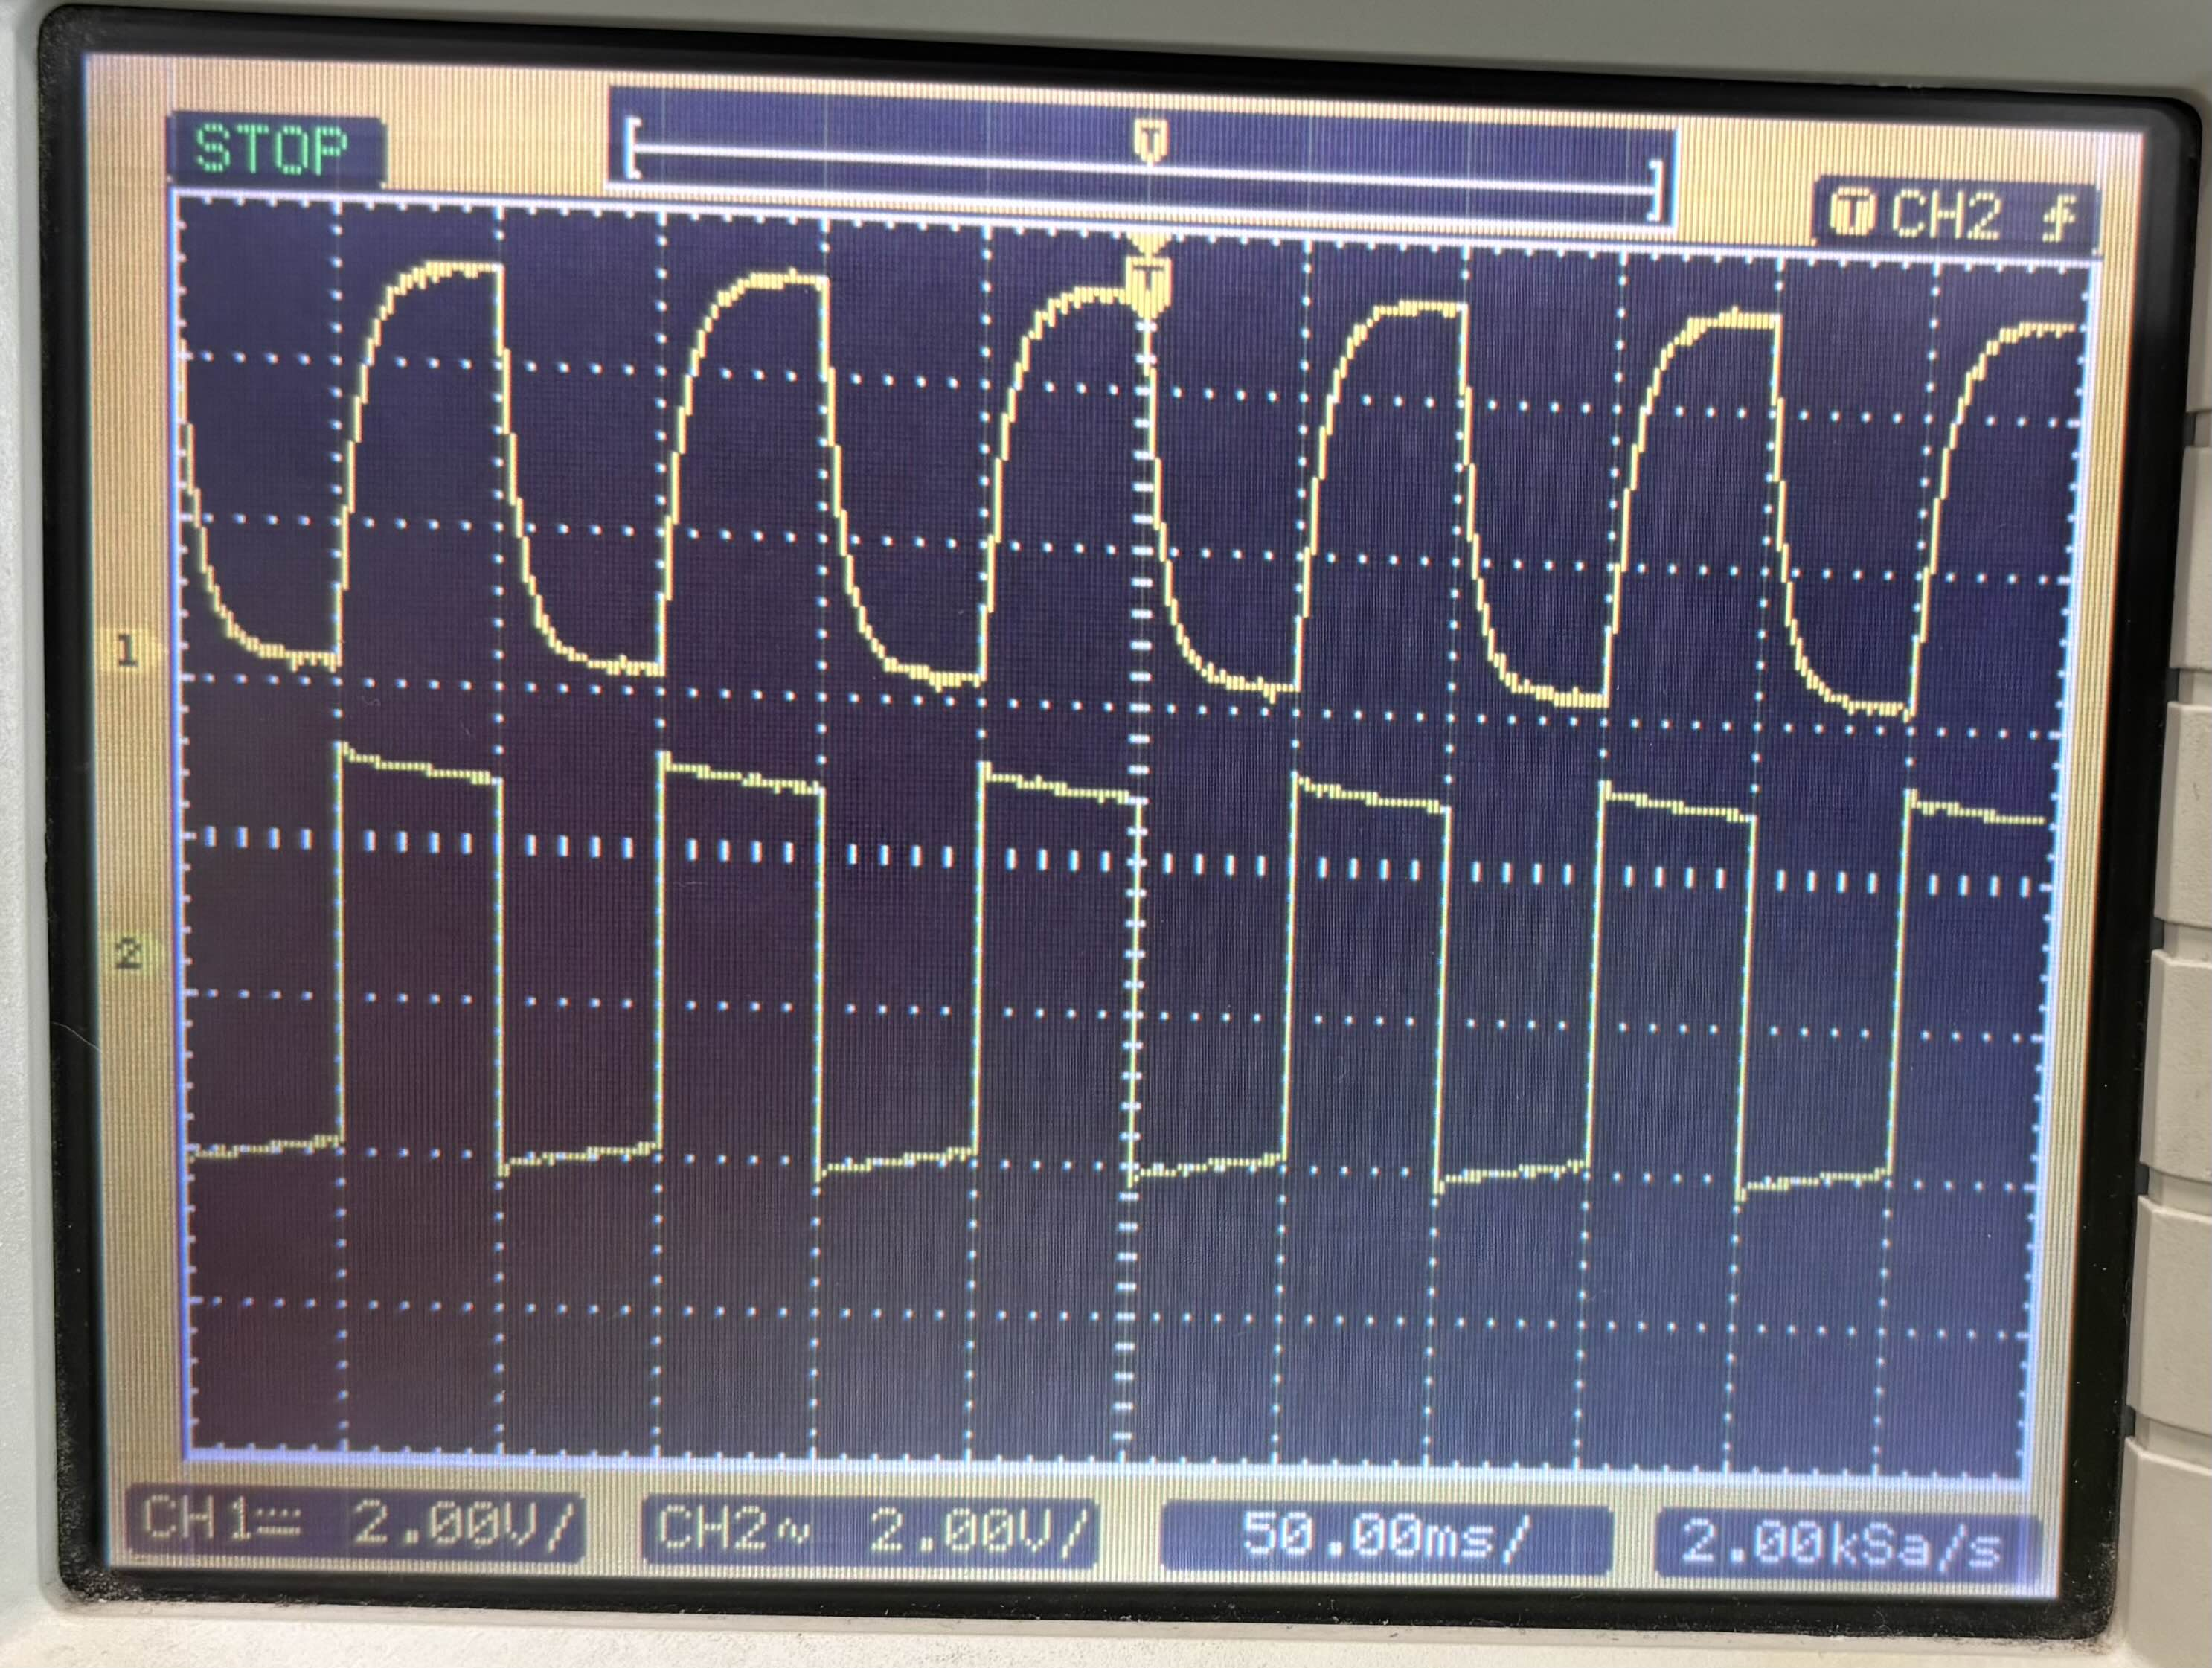
\includegraphics[width = 150pt]{figs/steady_1.jpg}
	\end{subfigure}
	\hspace{135pt}
	\begin{subfigure}[b]{10pt}
	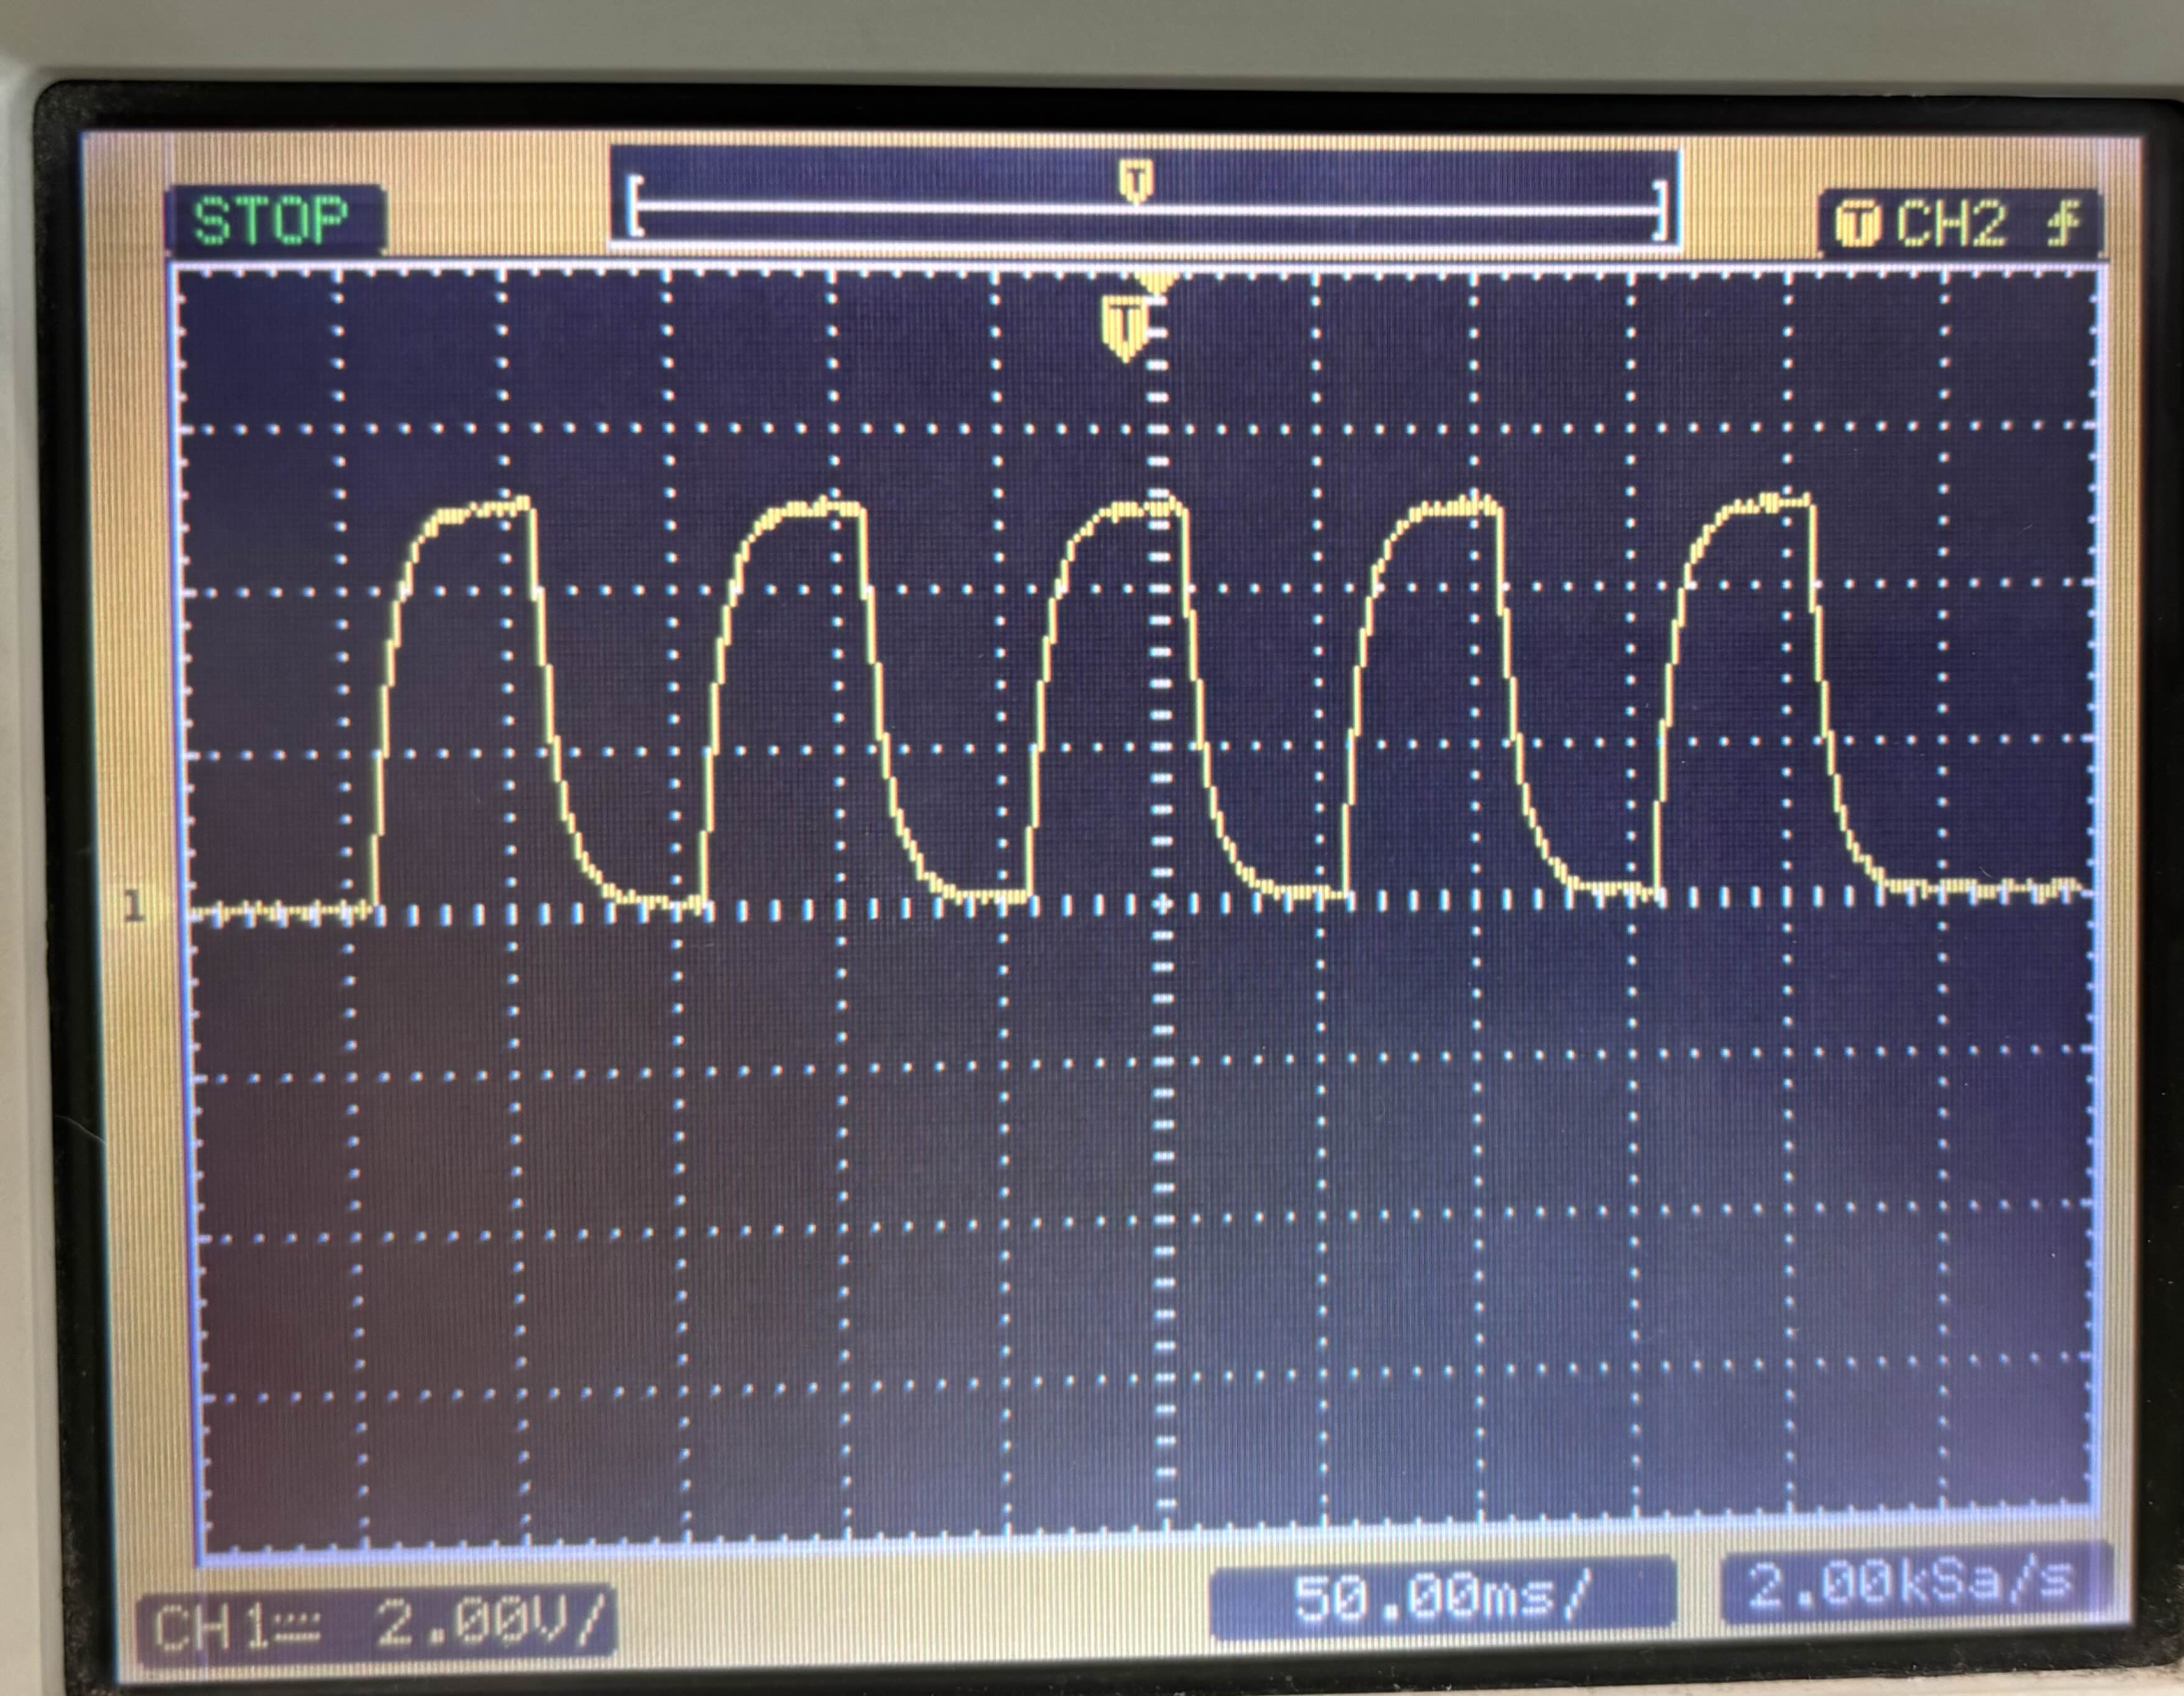
\includegraphics[width = 150pt]{./figs/trans_1.jpg}
	\end{subfigure}
	\hspace{135pt}
	\begin{subfigure}[b]{10pt}
	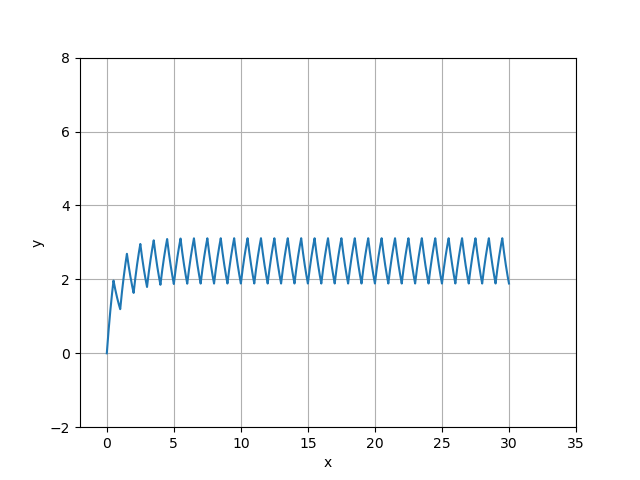
\includegraphics[width = 150pt]{./figs/fig1.png}
	\end{subfigure}
\end{figure*}
\subsection*{Case 2: $RC = T$}
When RC = T, the capacitor charges and discharges as the input wave alternates between 5 to 0V.
\begin{figure*}[h!]
	\begin{subfigure}[b]{10pt}
	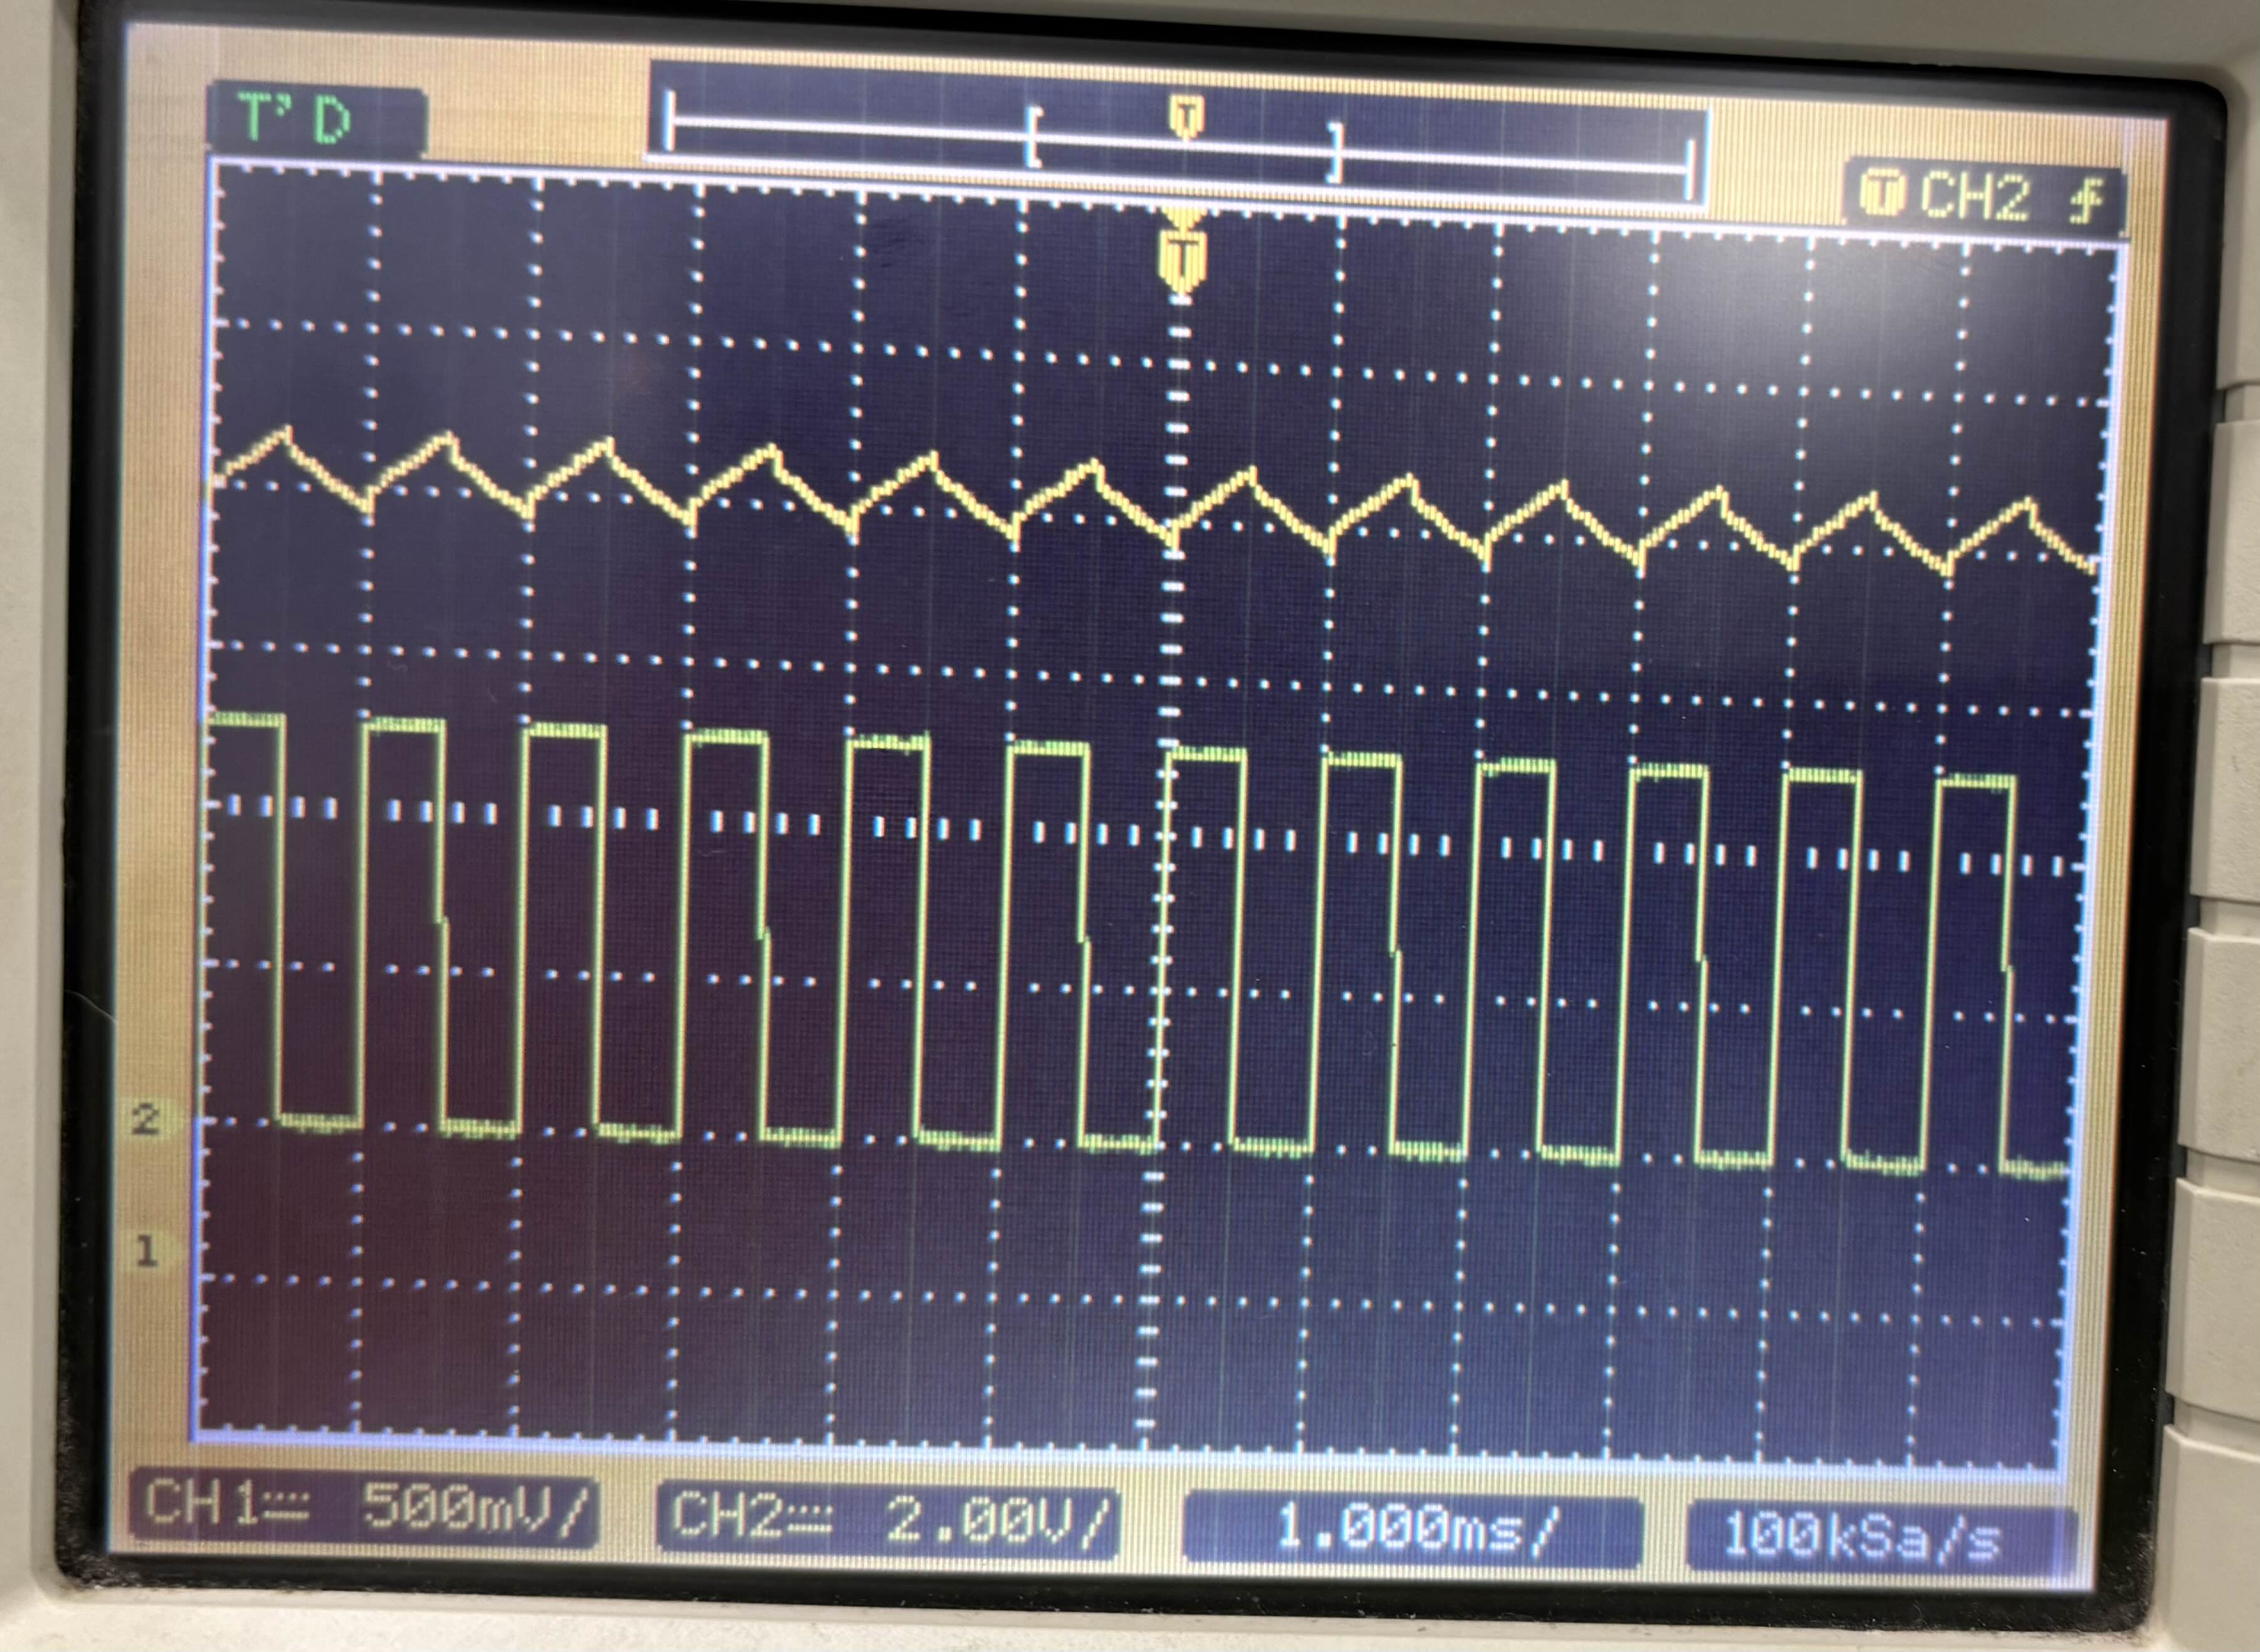
\includegraphics[ width = 150pt]{figs/steady_2.jpg}
	\end{subfigure}
	\hspace{135pt}
	\begin{subfigure}[b]{10pt}
	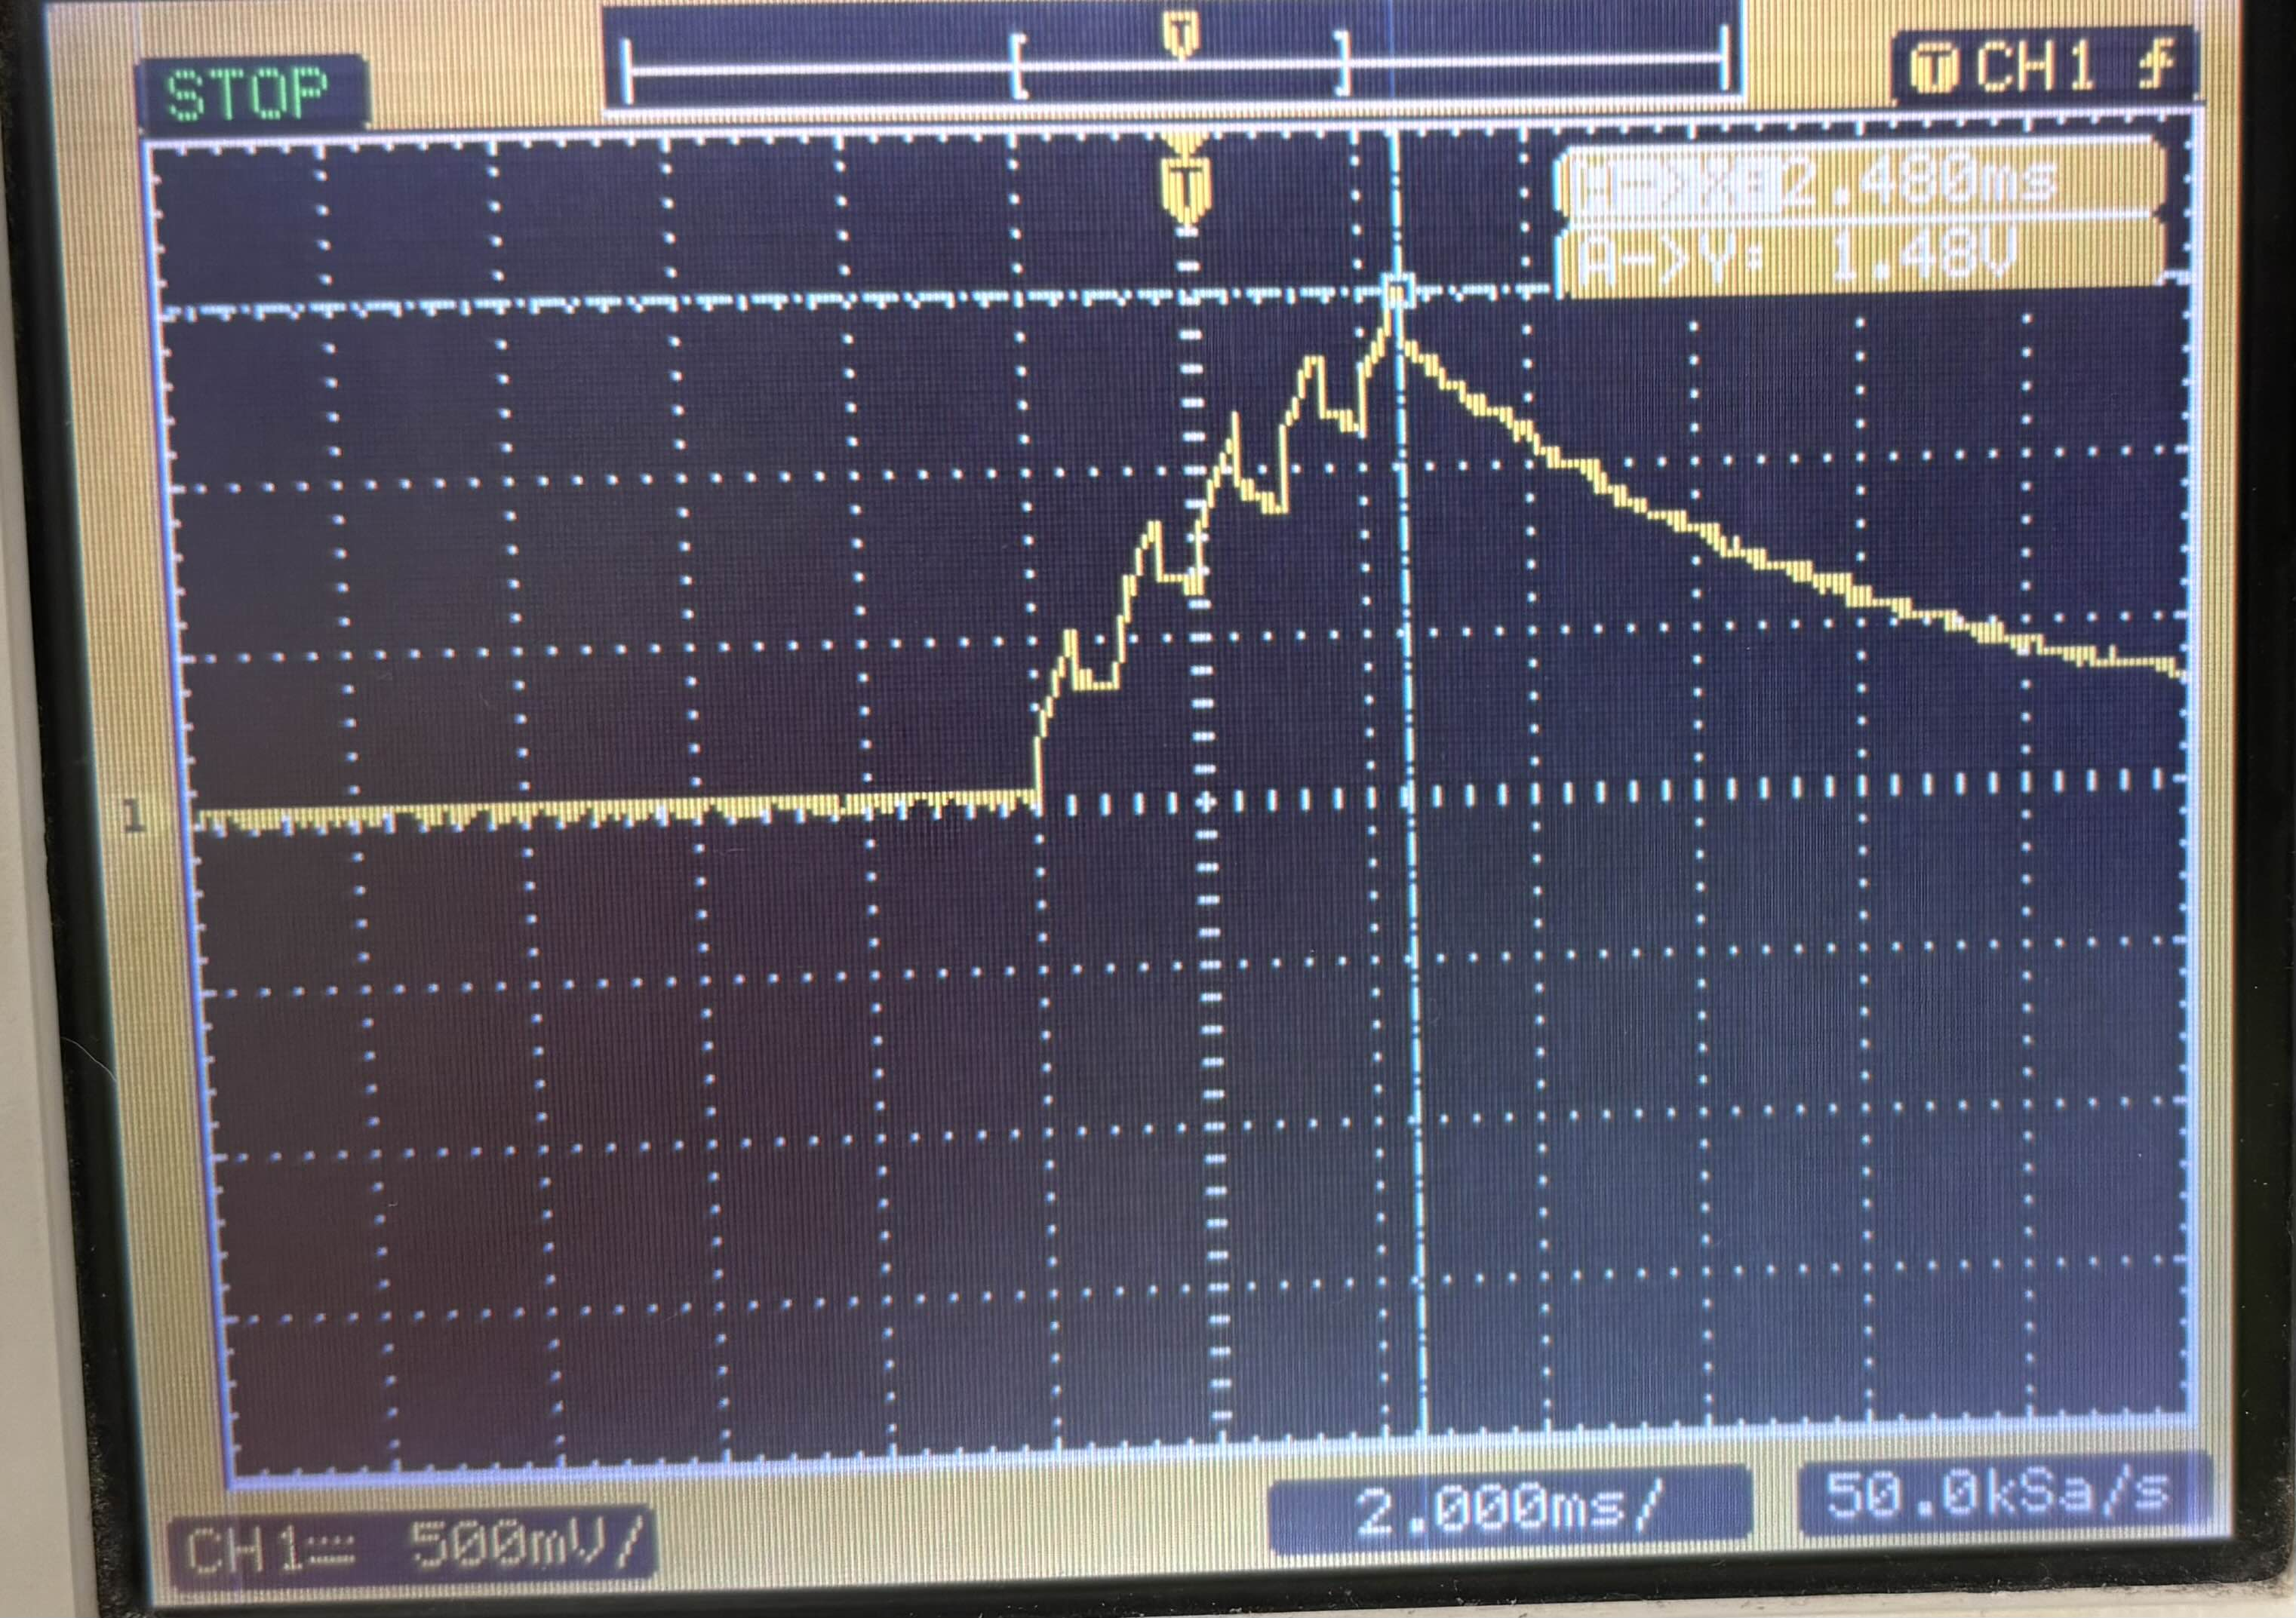
\includegraphics[ width = 150pt]{./figs/trans_2.jpg}
	\end{subfigure}
	\hspace{135pt}
	\begin{subfigure}[b]{10pt}
	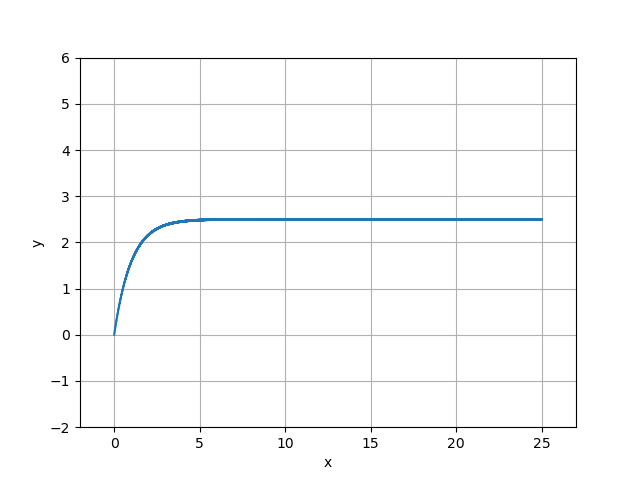
\includegraphics[ width = 150pt]{./figs/fig2.png}
	\end{subfigure}
\end{figure*}
\pagebreak
\subsection*{Case 3: $RC >> T$}
When RC is very large than T, the capacitor charges and discharges very slowly making the graph very smooth and almost like a response to a DC input.
Here, we have plotted more than $5$ cycles of square wave as it better shows the increasing nature of the potential difference across capacitor. 
\begin{figure*}[h!]
	\begin{subfigure}[b]{10pt}
	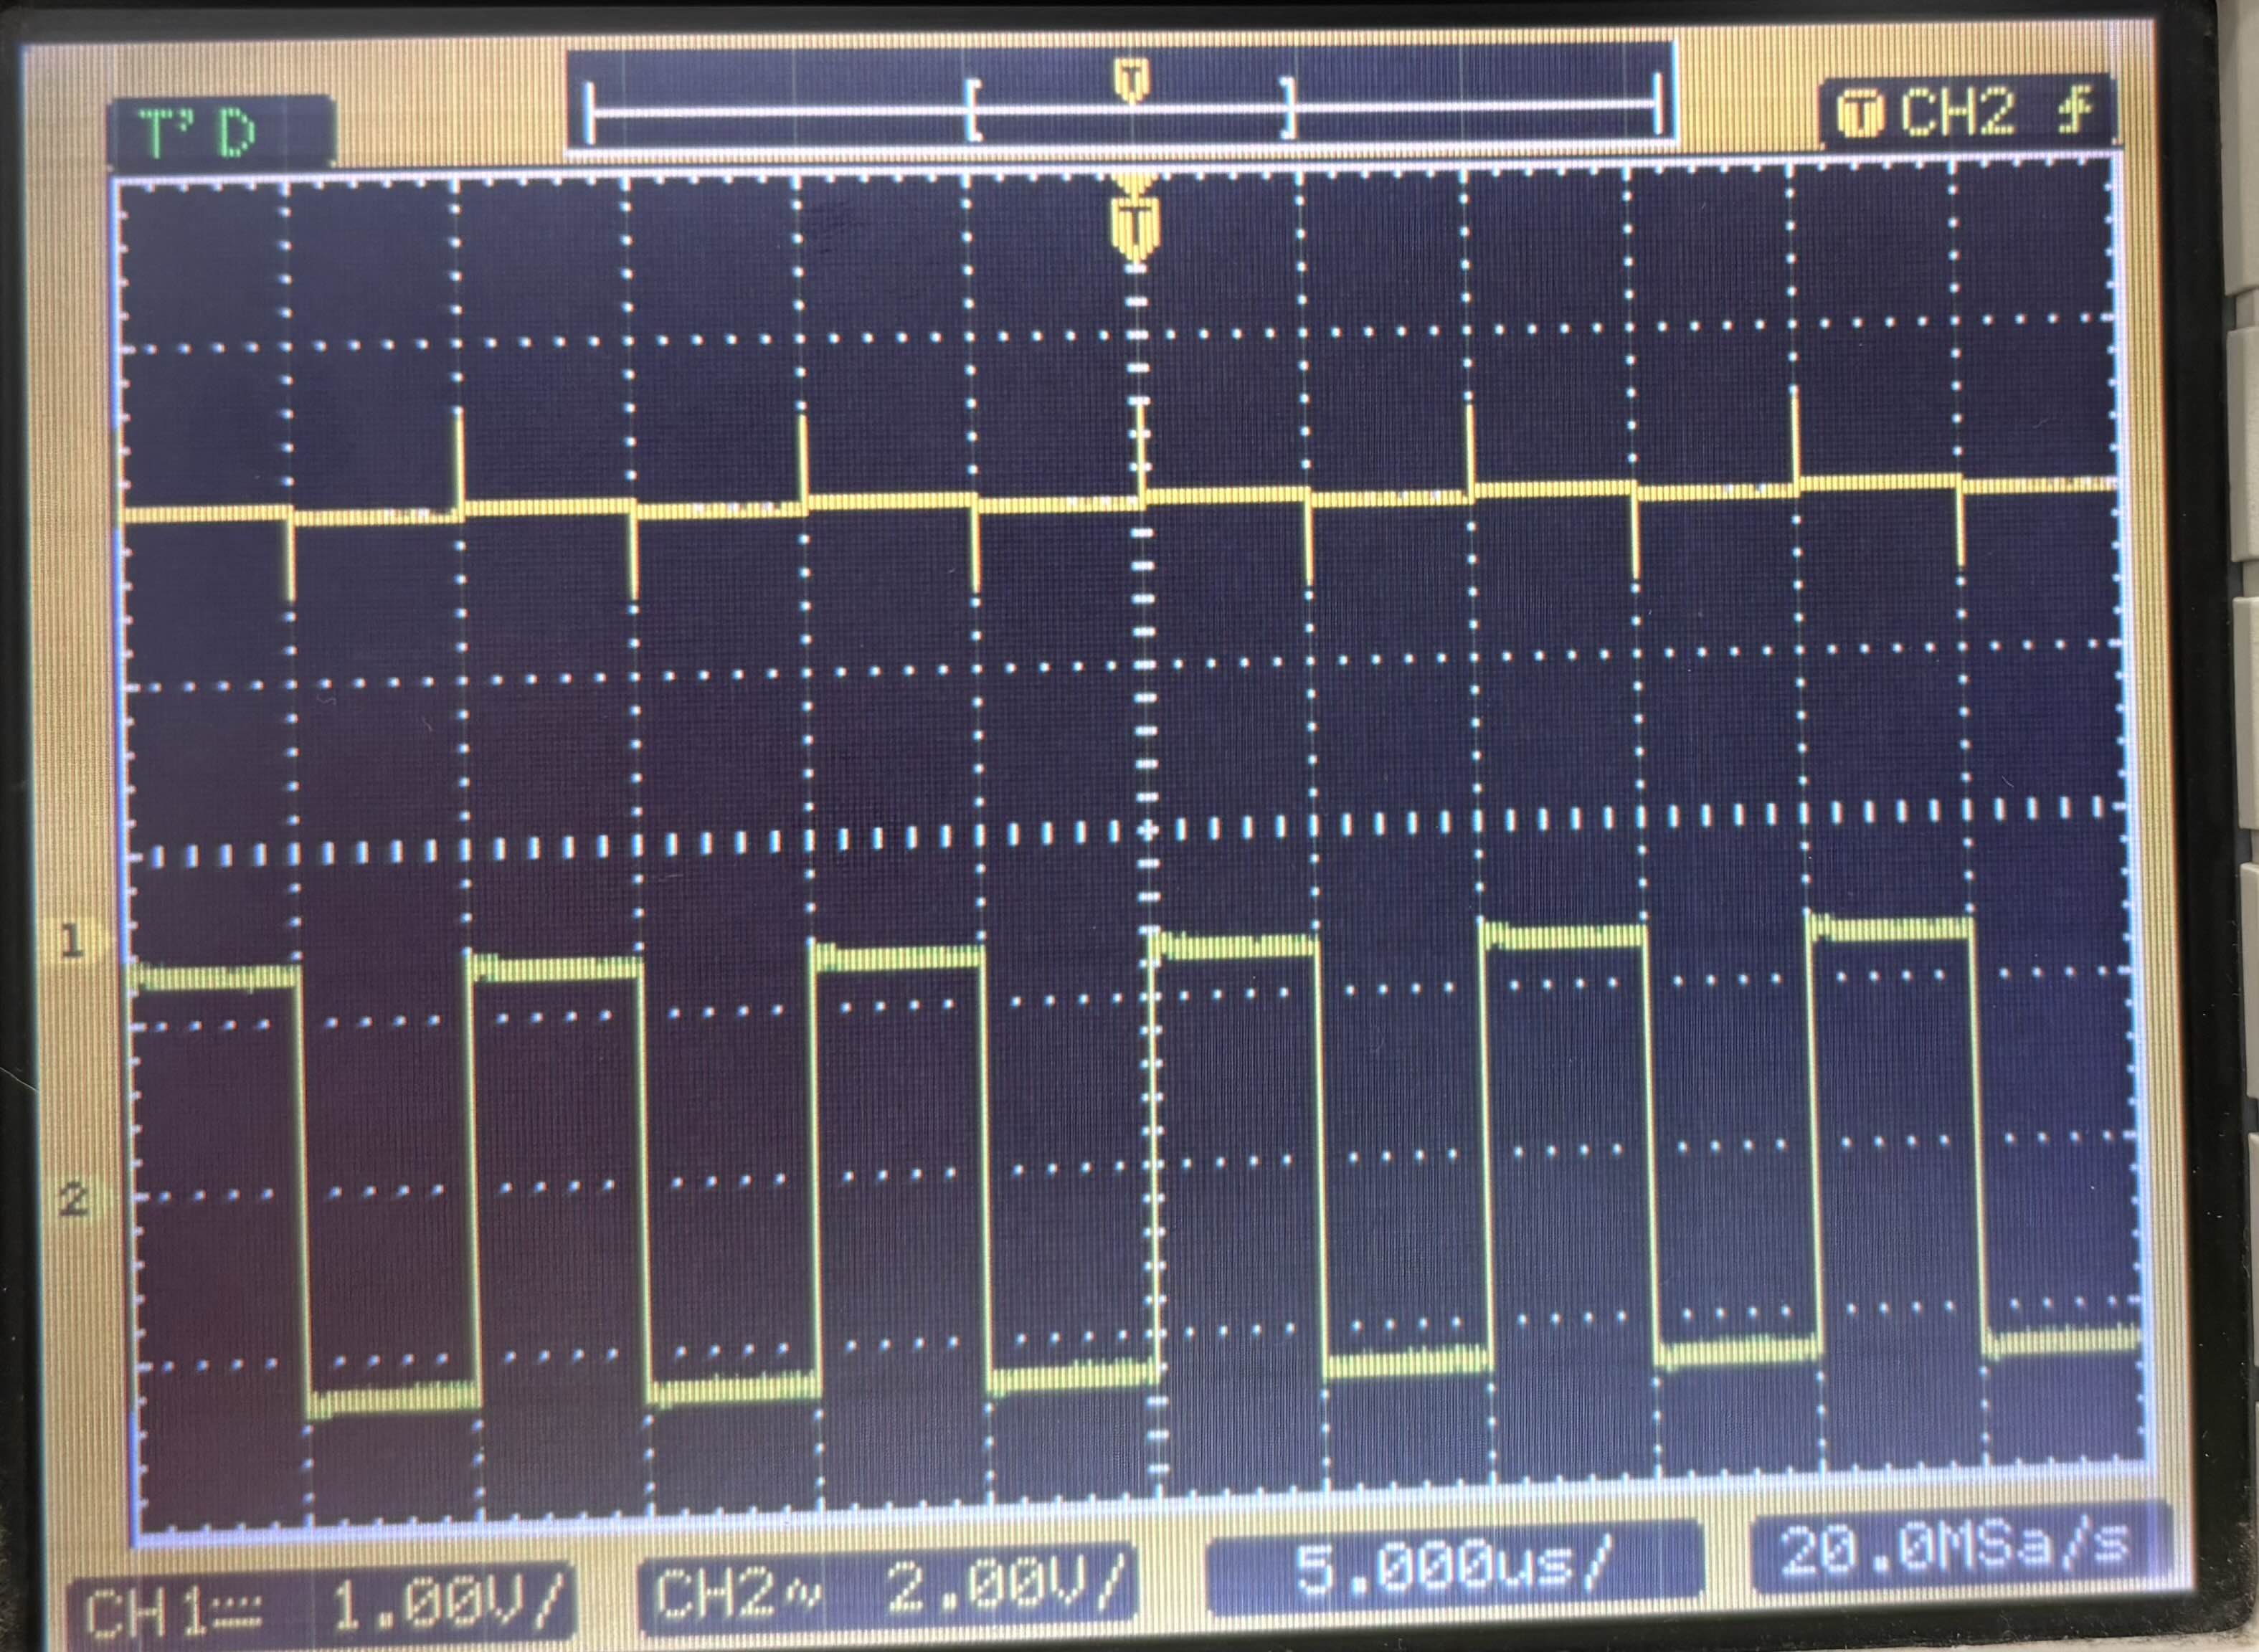
\includegraphics[ width = 150pt]{figs/steady_3.jpg}
	\end{subfigure}
	\hspace{135pt}
	\begin{subfigure}[b]{10pt}
	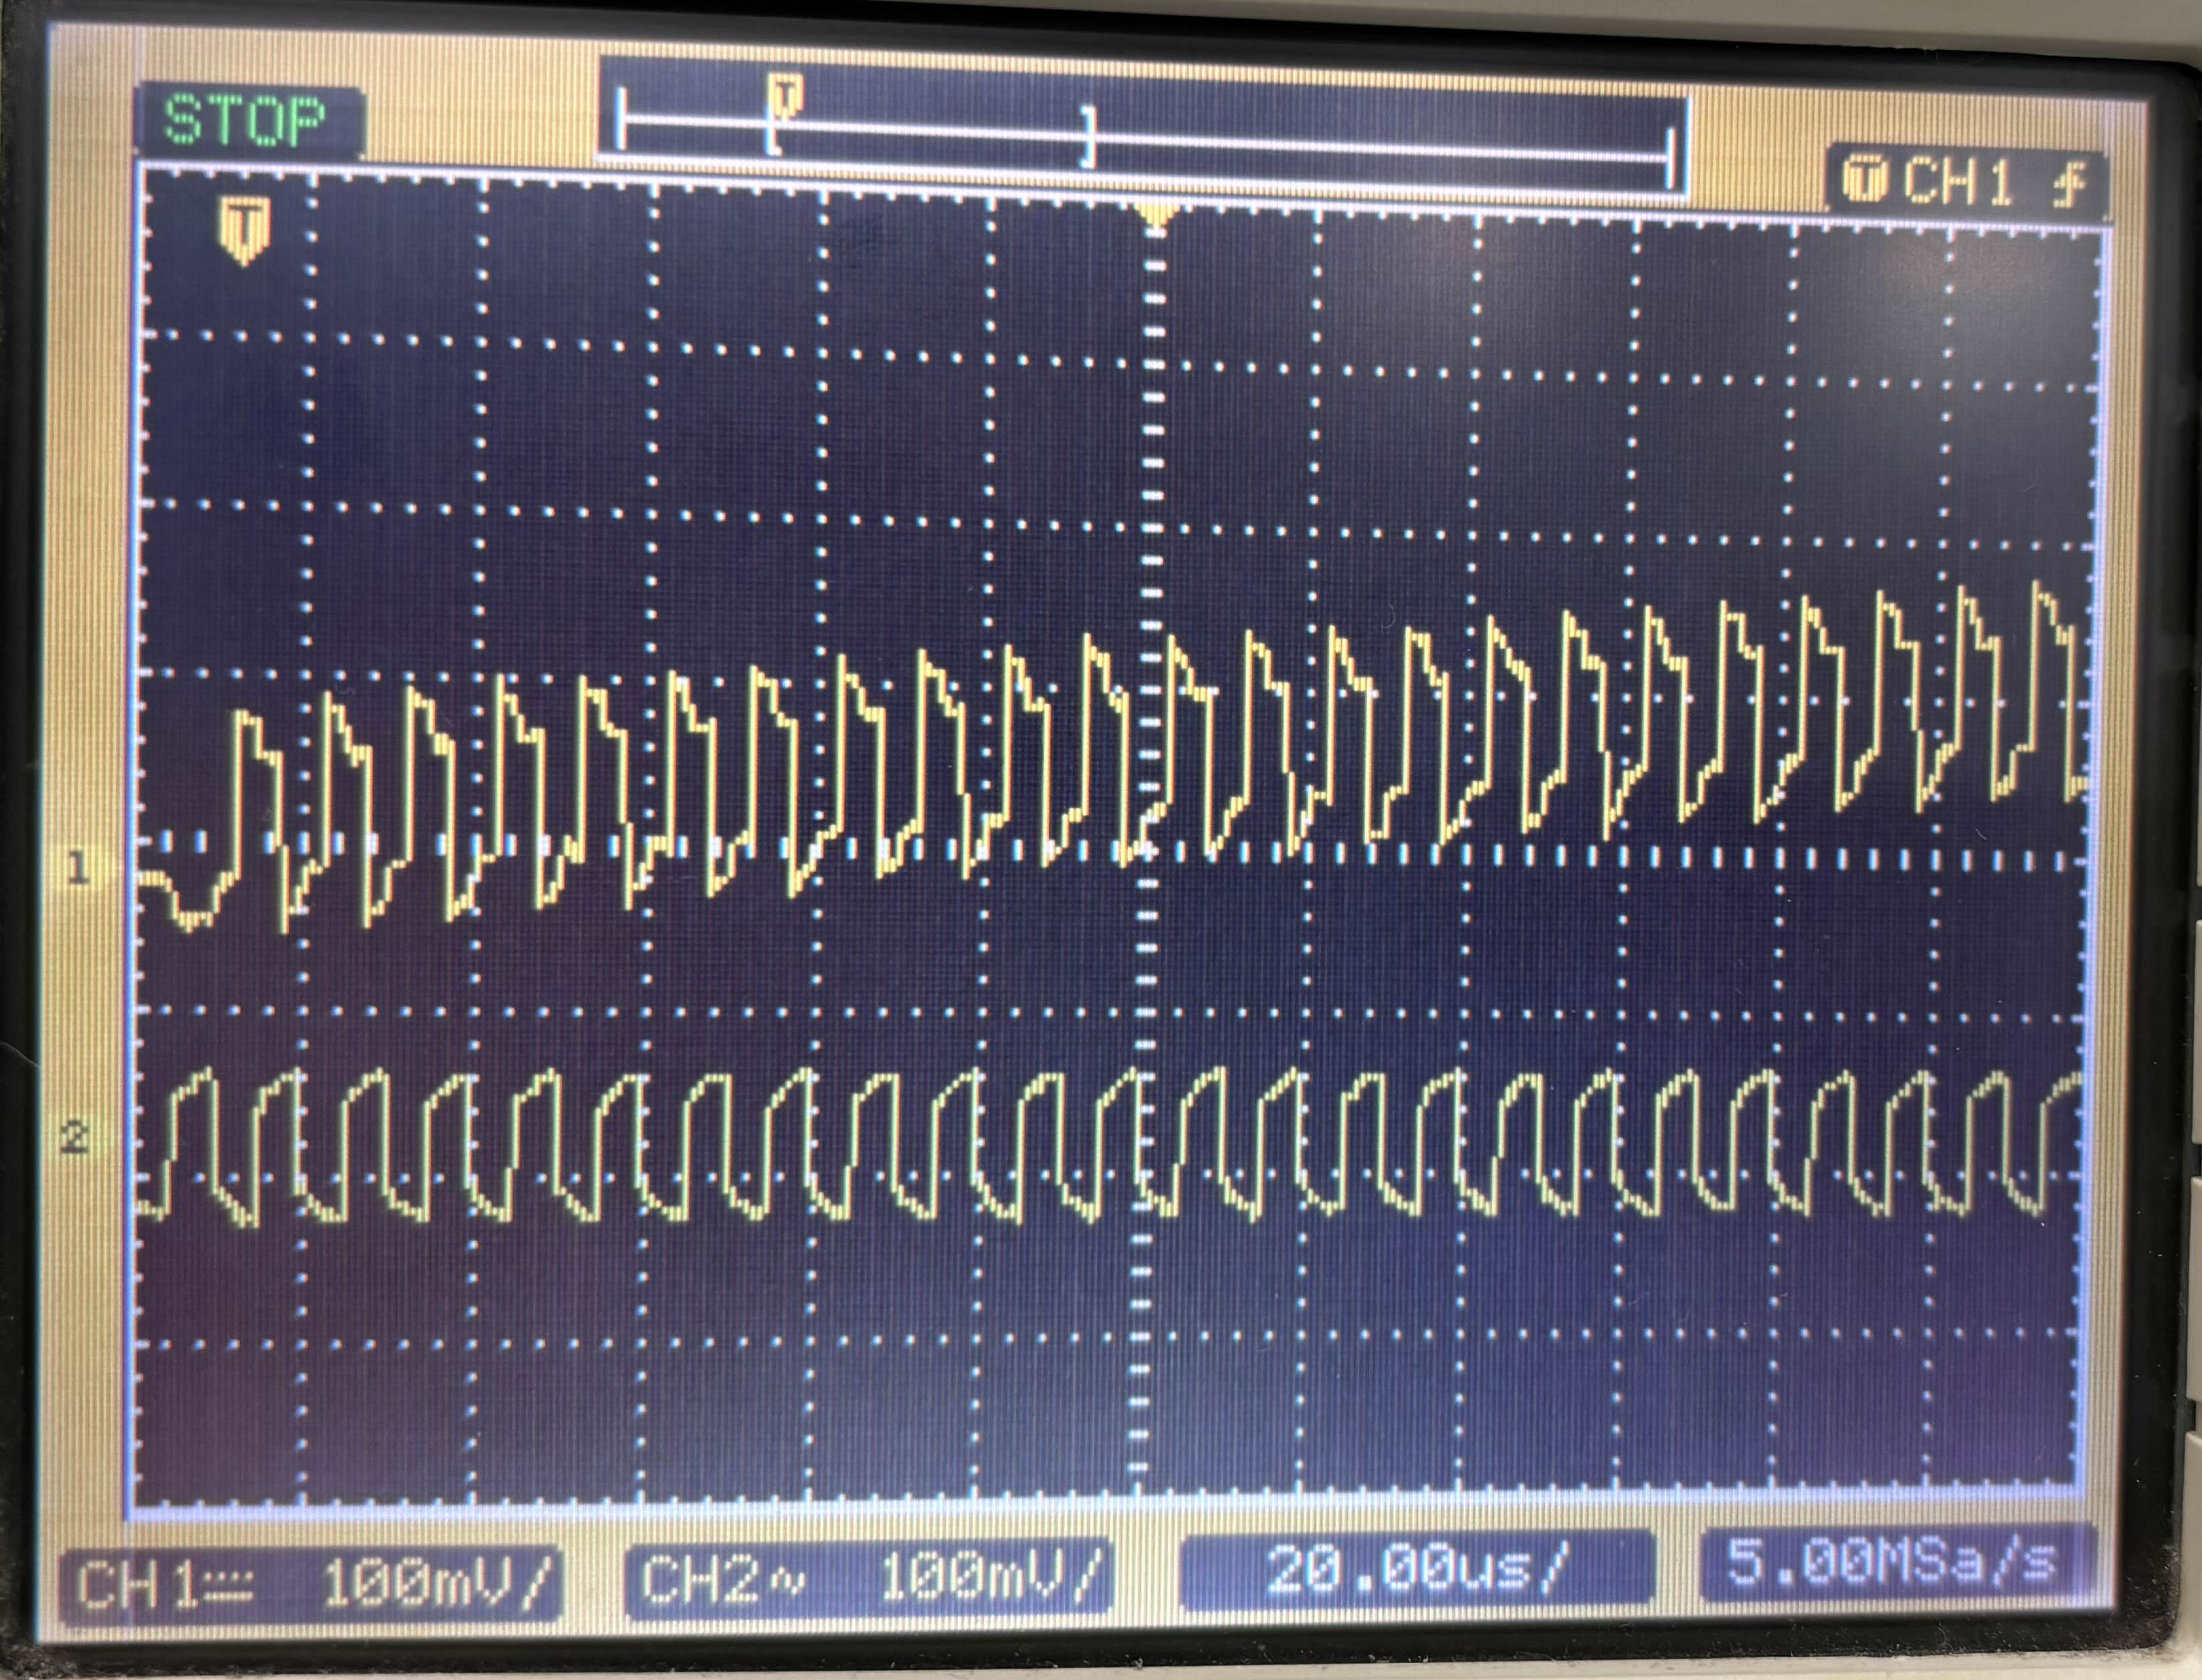
\includegraphics[ width = 150pt]{./figs/trans_3.jpg}
	\end{subfigure}
	\hspace{135pt}
	\begin{subfigure}[b]{10pt}
	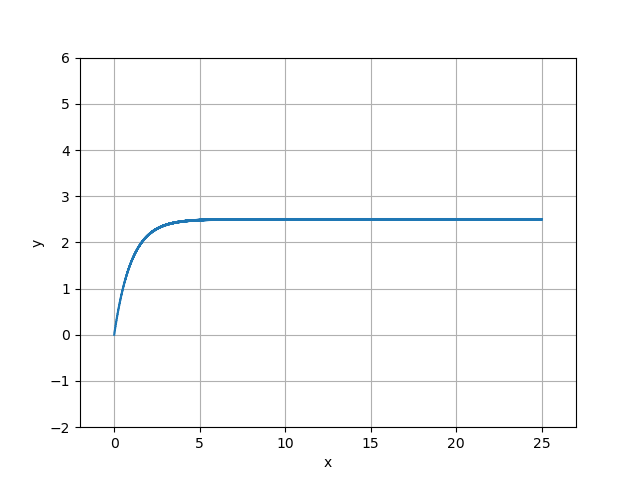
\includegraphics[ width = 150pt]{./figs/fig3.png}
	\end{subfigure}
\end{figure*}
For an infinite number of cycles of square wave, output comes out to be,
\begin{figure}[h!]
	\centering
	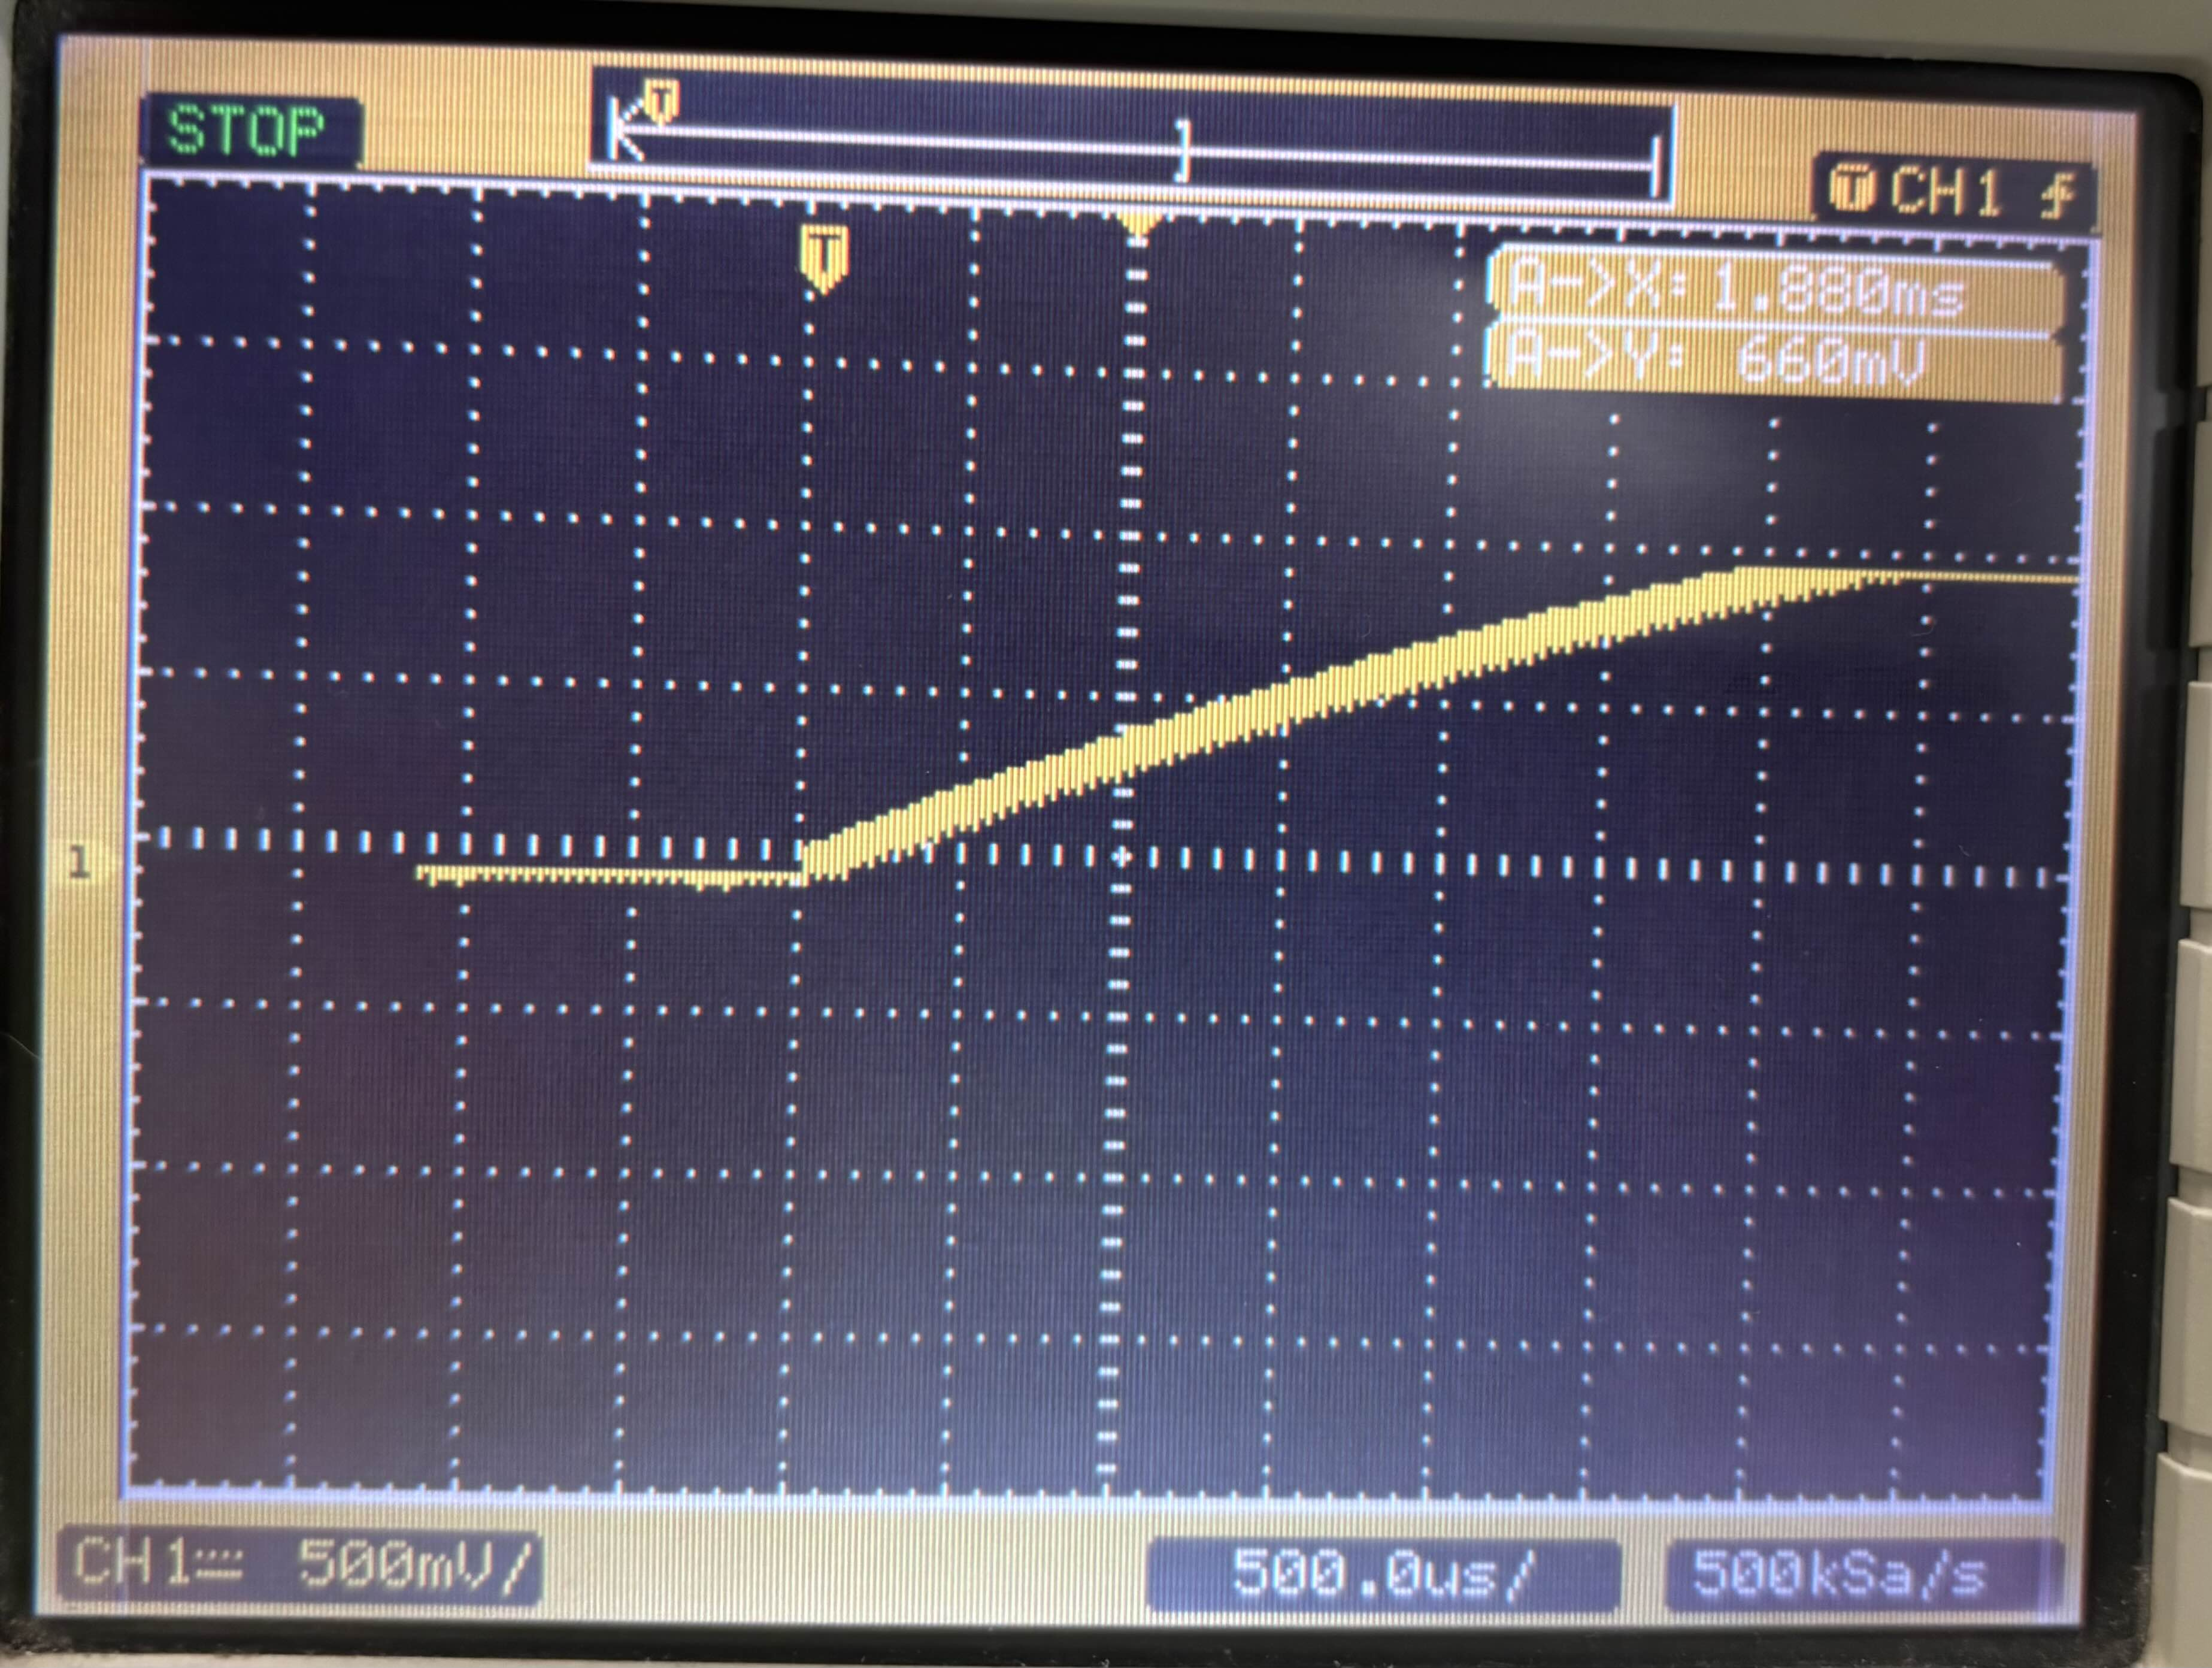
\includegraphics[width=0.7\columnwidth]{figs/trans_infty.jpg}
	\label{label}
\end{figure}\\
Python code verification of obtained graphs:\\
\fbox{\url{https://github.com/ArjunPavanje/EE1200/tree/main/Experiment_2/codes}}

\section*{Conclusion}
We have successfully found and verified the effect (output) of a square wave on a series RC circuit.
\end{document}
